% MECE 4305 -- Lecture 10 supplement (12 Nov 2026): ascentopt -- launch-trajectory / propulsion co-design
% Build: latexmk -pdf slides.tex   (needs beamercolorthemeColumbia.sty and figs/*.pdf from make_doc_figs.py)
% Frames are drop-in compatible with week10.tex (same theme, colours and macros); add {figs/} to its \graphicspath.
\documentclass[aspectratio=169,10pt]{beamer}
\usetheme{Madrid}
\usecolortheme{Columbia}
\setbeamertemplate{navigation symbols}{}
\setbeamertemplate{itemize items}[circle]
\setbeamertemplate{enumerate items}[default]
\setbeamertemplate{caption}{\raggedright\insertcaption\par}
\setbeamerfont{caption}{size=\scriptsize}
\setbeamerfont{footnote}{size=\tiny}
\setbeamersize{text margin left=7mm,text margin right=7mm}

\usepackage[T1]{fontenc}\usepackage{lmodern}
\usepackage{amsmath,amssymb,bm}
\usepackage{siunitx}
\usepackage{booktabs}
\usepackage{graphicx}
\usepackage[table]{xcolor}
\usepackage{tikz}
\usetikzlibrary{arrows.meta,positioning,calc,decorations.pathreplacing,fit,backgrounds}
\usepackage{hyperref}
\usepackage{tcolorbox}
\usepackage{listings}

\graphicspath{{figs/}}
\sisetup{per-mode=symbol,range-phrase=--,range-units=single}
\DeclareSIUnit{\tonne}{t}

% --- macros shared with week10.tex (providecommand so the frames can be pasted into that deck) ---
\providecommand{\Isp}{{I_{sp}}}\providecommand{\cstar}{{c^{*}}}\providecommand{\CF}{{C_F}}\providecommand{\mdot}{\dot m}
\providecommand{\dv}{\Delta v}\providecommand{\gz}{g_0}\providecommand{\pc}{p_c}\providecommand{\dd}{\mathrm{d}}\providecommand{\eps}{\varepsilon}
\providecommand{\src}[1]{\vfill\hfill{\tiny\color{gray}#1}}
\providecommand{\stepbox}[2]{\begin{tcolorbox}[colback=PMS284C!15,colframe=PMS280C,boxrule=0.5pt,left=3pt,right=3pt,top=0pt,bottom=0pt,arc=1pt,boxsep=1pt]\footnotesize\textbf{Design procedure, step #1:} #2\end{tcolorbox}}
\definecolor{okgreen}{RGB}{0,131,0}
\newcommand{\tool}{\texttt{ascentopt}}
\newcommand{\stat}[2]{{\color{PMS7635C}\textbf{\large #1}}\\[-1pt]{\scriptsize\color{gray}#2}}
\lstset{basicstyle=\ttfamily\scriptsize,breaklines=true,columns=fullflexible,backgroundcolor=\color{PMS284C!12},frame=single,framerule=0.2pt,rulecolor=\color{PMS280C}}

\title[Lecture 10 -- Trajectory Tool]{Lecture 10 Supplement -- \texttt{ascentopt}: Launch Trajectory \& Propulsion Co-Design}
\subtitle{Mechanics \& Thermodynamics of Propulsion (MECE 4305)}
\author{David E. Tew, Ph.D.}
\institute[Columbia]{Columbia University \quad\textbullet\quad david.tew@columbia.edu}
\date{12 November 2026}

\begin{document}

% =====================================================================
\begin{frame}
  \titlepage
\end{frame}

\begin{frame}{Why a Trajectory Optimizer}
  \framesubtitle{A forward simulation flies a prescribed law; design needs the law solved for}
  \begin{columns}[T]
    \begin{column}{0.52\textwidth}
      \textbf{The usual first look} at a launch is a 3-DOF forward simulation: vertical rise, then a gravity turn (thrust along velocity). One stage, prescribed steering, no constraints, no objective.
      \begin{itemize}
        \item it answers ``where does this law go?'' -- not ``what is the most this vehicle can do?'';
        \item the loss rule of thumb, $\dv_{loss}\approx$ \SIrange{1.5}{2.0}{km/s}, is a band, not a number;
        \item a design needs: payload for a \emph{given} vehicle, the staging point, the loss breakdown, and the propulsion requirements $T$, $\Isp$, $\mdot$, burn time for the thrust-chamber and cycle steps.
      \end{itemize}
      \vspace{3pt}
      \textbf{What is needed:} trajectory optimization with a multistage vehicle model -- that is \tool.
    \end{column}
    \begin{column}{0.46\textwidth}
      \begin{block}{Hand method vs.\ the Starship Block 3 deck (dry 200/100 t)}
        \scriptsize
        \begin{tabular}{lcc}
          \toprule
          assumed $\dv_{req}$ & loss assumption & payload \\
          \midrule
          \SI{8800}{m/s} & \SI{1.5}{km/s} & \SI{339}{\tonne} \\
          \SI{9300}{m/s} & \SI{2.0}{km/s} & \SI{276}{\tonne} \\
          \rowcolor{PMS284C!25} \textbf{\SI{9155}{m/s}} & \textbf{optimizer: \SI{1833}{m/s}} & \textbf{\SI{293}{\tonne}} \\
          \bottomrule
        \end{tabular}\\[3pt]
        The trajectory decides the loss; the loss decides the payload. The band is worth $\pm\SI{30}{\tonne}$ here.
      \end{block}
    \end{column}
  \end{columns}
\end{frame}

% =====================================================================
\section{Method}
\begin{frame}{What \texttt{ascentopt} Is}
  \framesubtitle{3-DOF ascent physics -- steering and throttle become unknowns, the orbit a constraint, payload the objective}
  \centering
  \resizebox{\textwidth}{!}{%
  \begin{tikzpicture}[node distance=4mm and 5mm, font=\small,
    box/.style={draw, rounded corners=2pt, align=center, minimum height=9mm, inner sep=4pt, fill=PMS284C!15},
    red/.style={box, draw=PMS7635C, thick}, blue/.style={box, draw=PMS280C, thick},
    arr/.style={-{Latex[length=2.5mm]}, thick, gray}]
    \node[box] (deck) {vehicle deck (YAML)\\stages, engines, reserves};
    \node[box, below=of deck] (mis) {mission\\orbit, site, $q_{max}$, $a_{max}$};
    \node[blue, right=9mm of $(deck.east)!0.5!(mis.east)$] (guess) {gravity-turn\\initial guess\\(prescribed law)};
    \node[red, right=of guess] (nlp) {Dymos trajectory\\phases, controls,\\linkages, constraints};
    \node[red, right=of nlp] (ipopt) {IPOPT\\(sparse NLP,\\coloured Jacobian)};
    \node[blue, right=of ipopt] (ver) {verification\\explicit re-integration\\loss identity, grid};
    \node[box, right=of ver] (out) {outputs\\histories, staging,\\losses, $T$, $\Isp$, $\mdot$};
    \draw[arr] (deck.east) -- ++(4mm,0) |- (guess.west);
    \draw[arr] (mis.east) -- ++(4mm,0) |- (guess.west);
    \draw[arr] (guess) -- (nlp); \draw[arr] (nlp) -- (ipopt); \draw[arr] (ipopt) -- (ver); \draw[arr] (ver) -- (out);
    \draw[arr, dashed] (ipopt.south) -- ++(0,-6mm) -| node[pos=0.25, below, font=\footnotesize]{warm start / restart, deck overrides (sweeps)} (nlp.south);
    \begin{scope}[on background layer]
      \node[draw=gray, dashed, rounded corners, fit=(nlp)(ipopt), inner sep=5pt, label={[font=\footnotesize, gray]above:OpenMDAO problem (jax ODE, automatic derivatives)}] {};
    \end{scope}
  \end{tikzpicture}}
  \vspace{4pt}
  \begin{columns}[T]
    \begin{column}{0.48\textwidth}
      \begin{block}{Physics (as in a forward simulation)}
        \footnotesize 3-DOF point mass, rotating Earth, atmosphere and drag, back-pressure thrust law; a prescribed gravity-turn law supplies the initial guess and an independent check.
      \end{block}
    \end{column}
    \begin{column}{0.48\textwidth}
      \begin{block}{Added}
        \footnotesize Controls $\hat{\bm u}(t)$, $\tau(t)$; phases linked at staging; path and terminal constraints; max-payload objective; five loss accumulators; sweeps by deck override.
      \end{block}
    \end{column}
  \end{columns}
\end{frame}

\begin{frame}{Physical Model}
  \framesubtitle{Point mass in an Earth-centred inertial frame; drag on the air-relative velocity}
  \begin{columns}[T]
    \begin{column}{0.46\textwidth}
      \centering
      \begin{tikzpicture}[scale=0.85, font=\footnotesize, >={Latex[length=2.2mm]}]
        \fill[PMS284C!25] (0,0) circle (1.5); \draw[PMS284C, thick] (0,0) circle (1.5);
        \node[PMS280C] at (0,-0.3) {Earth}; \draw[->, gray] (0,0) -- (0,0.95) node[right] {$\bm\omega$};
        \coordinate (P) at (3.1,2.2);
        \draw[->, dashed, gray] (0,0) -- (P) node[midway, below right] {$\bm r$};
        \fill[black] (P) circle (0.06);
        \draw[->, thick, PMS2461C] (P) -- ++(1.5,1.0) node[above] {$\bm v$};
        \draw[->, thick, PMS7635C] (P) -- ++(1.8,0.45) node[right] {$T\hat{\bm u}$};
        \draw[->, thick, orange!80!black] (P) -- ++(-1.0,-0.7) node[below] {$D\hat{\bm v}_{rel}$};
        \draw[->, thick, black] (P) -- ($(P)!0.45!(0,0)$) node[pos=0.6, right=2pt] {$-\mu m\bm r/r^3$};
        \draw[->, gray, thin] (P) -- ++(0.55,0.9) node[above] {$\hat{\bm r}$};
      \end{tikzpicture}
    \end{column}
    \begin{column}{0.54\textwidth}
      \small
      \begin{align*}
        \dot{\bm r} &= \bm v \\
        \dot{\bm v} &= -\tfrac{\mu}{r^3}\bm r + \tfrac{T}{m}\hat{\bm u} - \tfrac{D}{m}\hat{\bm v}_{rel},\qquad \bm v_{rel} = \bm v - \bm\omega\times\bm r\\
        \dot m_p &= -\tau\,\mdot_{max},\qquad T = \tau\,\bigl(T_{vac} - p_a(h)A_e\bigr),\qquad D = \tfrac12\rho(h)|\bm v_{rel}|^2 C_D A_{ref}
      \end{align*}
      \begin{itemize}
        \item ECI Cartesian: no polar singularity, no trigonometry in the dynamics
        \item $\bm v_0 = \bm\omega\times\bm r_0$: the \SI{418}{m/s} rotation credit falls out -- no separately signed term to get wrong
        \item drag on the \emph{air-relative} velocity, not the inertial velocity
        \item loss rates $g\sin\gamma$, $D/m$, $(T/m)(1-\cos\alpha_T)$, $\tau p_aA_e/m$ integrated as extra states
      \end{itemize}
    \end{column}
  \end{columns}
\end{frame}

\begin{frame}{Environment and Engine Models}
  \framesubtitle{US Standard Atmosphere 1976 as a smooth table; one anchor pair per engine}
  \begin{columns}[T]
    \begin{column}{0.5\textwidth}
      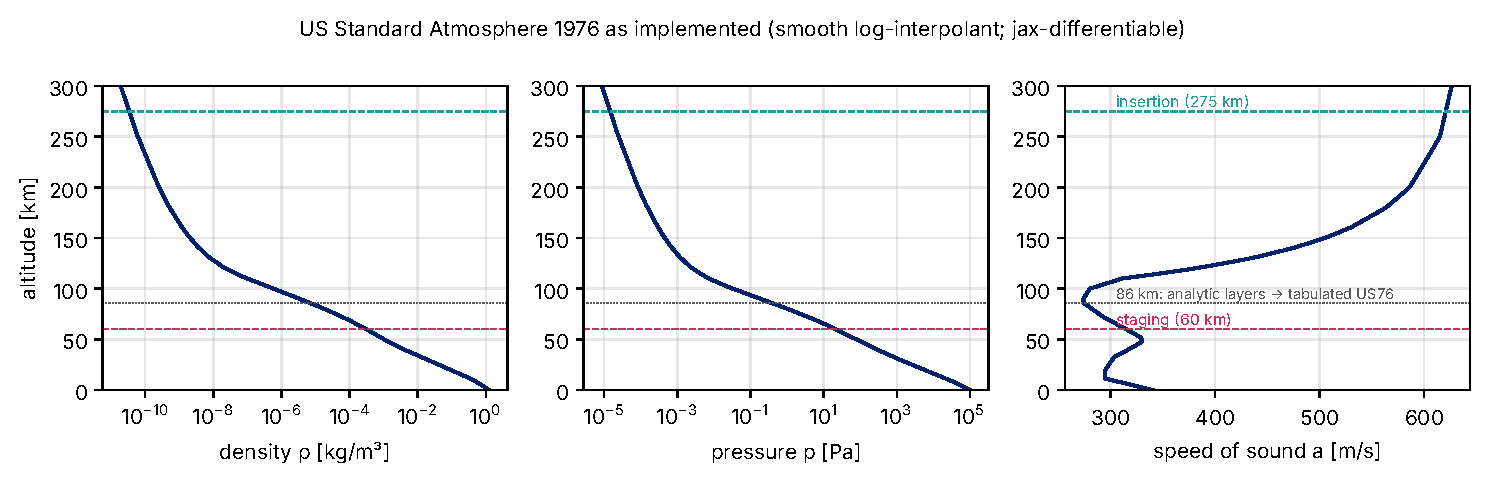
\includegraphics[width=\textwidth]{fig_atmosphere}\\
      {\footnotesize Analytic layers to \SI{86}{km}, tabulated above, log-interpolated $\Rightarrow$ differentiable to orbit. Matches the \texttt{ambiance} ISA package to $<0.1\,\%$ below \SI{81}{km}.}
    \end{column}
    \begin{column}{0.5\textwidth}
      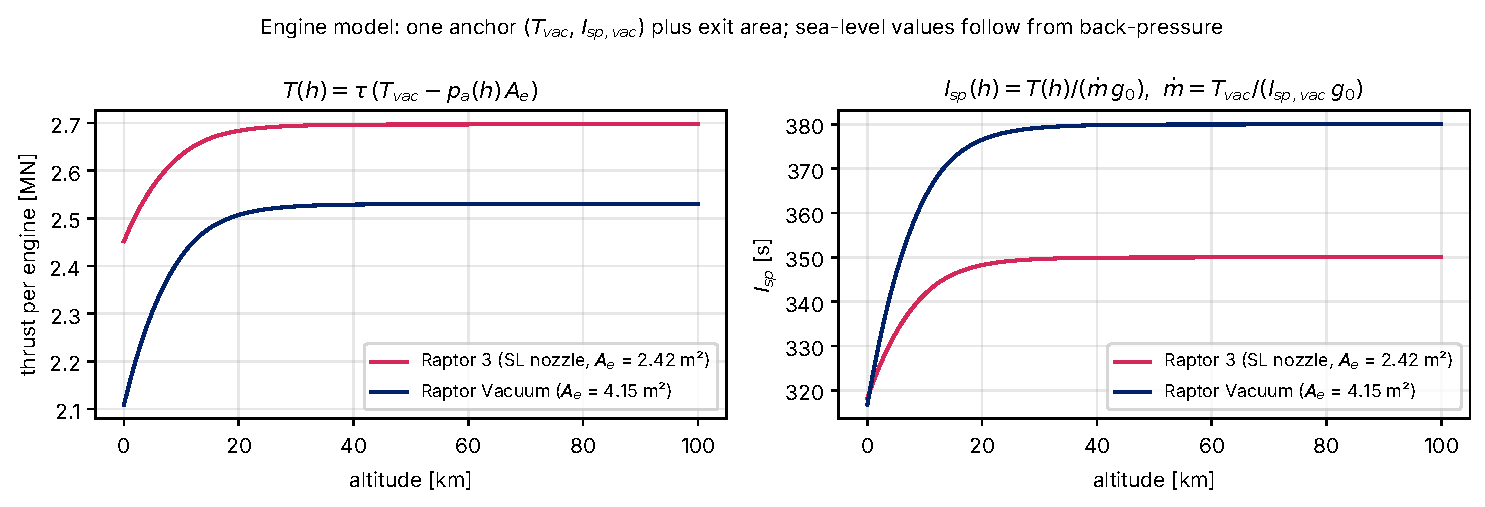
\includegraphics[width=\textwidth]{fig_engine_model}\\
      {\footnotesize $(T_{vac}, \Isp_{,vac})$ + exit area; sea-level values are \emph{outputs}. Published Raptor pairs from different sources are not mutually consistent (\SI{258}{tf} vac would need a \SI{1.86}{m} exit) -- a model, not a lookup.}
    \end{column}
  \end{columns}
\end{frame}

\begin{frame}{The Optimal-Control Problem}
  \framesubtitle{Maximize payload; one phase per burn, propellant a separate state per stage}
  \small
  \begin{tabular}{lp{10.6cm}}
    \toprule
    maximize & $m_{pay}$ \quad (or: minimize propellant, minimize time) \\
    over & $\hat{\bm u}(t)$, $\tau(t)$ per burn phase; phase durations; $m_{pay}$ \\
    dynamics & collocation defects in every phase \\
    path & $|\bm u|^2=1$,\; $0.4\le\tau\le1$,\; $h\ge0$,\; $q\le\SI{35}{kPa}$,\; $T/m\le4\,\gz$ \\
    linkage & $t,\bm r,\bm v$ and loss states continuous between phases; $m_p$ is \emph{not} linked \\
    boundary & $m_p$ = stage load at ignition; $m_p(t_f)\ge m_{reserve}$ at burnout \\
    terminal & $h=\SI{275}{km}$,\; $\gamma=0$,\; $|\bm v|=\sqrt{\mu/r}$ \;[, $i=i_{target}$] \\
    \bottomrule
  \end{tabular}
  \vspace{4pt}
  \centering
  \resizebox{0.95\textwidth}{!}{%
  \begin{tikzpicture}[font=\small, >={Latex[length=2.3mm]},
    ph/.style={draw, thick, rounded corners=2pt, minimum height=13mm, align=center, fill=PMS284C!15}]
    \node[ph, draw=gray, minimum width=17mm] (rise) {\textbf{rise}\\10~s vertical\\$\hat{\bm u}=\hat{\bm r}$, $\tau=1$};
    \node[ph, draw=PMS7635C, minimum width=50mm, right=17mm of rise] (b) {\textbf{stage0} --- Super Heavy, 33 Raptor~3\\controls $\hat{\bm u},\tau$; $q\le q_{max}$, $T/m\le a_{max}$\\$m_p$: 3,650 t $\to$ reserve};
    \node[ph, draw=PMS280C, minimum width=62mm, right=17mm of b] (s) {\textbf{stage1} --- Starship, 3 Raptor~3 + 3 RVac\\controls $\hat{\bm u},\tau$; $T/m\le a_{max}$\\$m_p$: 1,600 t $\to$ reserve; orbit constraints};
    \draw[->, gray, thick] (rise) -- node[above=7.5mm, font=\scriptsize]{link: $t,\bm r,\bm v,L_\ast,m_p$} (b);
    \draw[->, gray, thick] (b) -- node[above=7.5mm, font=\scriptsize]{link: $t,\bm r,\bm v,L_\ast$ (not $m_p$)} (s);
  \end{tikzpicture}}
  \stepbox{0--4}{mission $\to$ $\dv$ $\to$ propellant fraction $\to$ required $\Isp$ $\to$ staging, solved as one problem with the trajectory in the loop.}
\end{frame}

\begin{frame}{Direct Collocation in \texttt{ascentopt}}
  \framesubtitle{Radau pseudospectral transcription, exact sparse derivatives, IPOPT}
  \begin{columns}[T]
    \begin{column}{0.55\textwidth}
      \begin{tikzpicture}[font=\footnotesize, >={Latex[length=2mm]}, xscale=0.62, yscale=0.9]
        \draw[->] (0,0) -- (10.6,0) node[right] {$t$};
        \foreach \x in {0,3.5,7,10} \draw[thick] (\x,-0.12) -- (\x,0.12);
        \node[below] at (1.75,-0.15) {segment 1}; \node[below] at (5.25,-0.15) {segment 2}; \node[below] at (8.5,-0.15) {segment $n$};
        \draw[PMS280C, thick] plot[smooth] coordinates {(0,0.6) (1.2,1.1) (2.4,1.35) (3.5,1.5)};
        \draw[PMS280C, thick] plot[smooth] coordinates {(3.5,1.5) (4.7,1.75) (5.9,2.05) (7,2.2)};
        \draw[PMS280C, thick] plot[smooth] coordinates {(7,2.2) (8,2.35) (9,2.5) (10,2.55)};
        \foreach \x/\y in {0/0.6, 0.65/0.95, 2.0/1.3, 3.5/1.5, 4.15/1.65, 5.5/2.0, 7/2.2, 7.6/2.3, 8.9/2.48, 10/2.55} \fill[PMS280C] (\x,\y) circle (0.07);
        \foreach \x/\y in {0.65/0.95, 2.0/1.3, 4.15/1.65, 5.5/2.0, 7.6/2.3, 8.9/2.48} \draw[PMS7635C, ->, thick] (\x,\y+0.45) -- (\x,\y+0.08);
        \node[PMS7635C, align=left] at (5.0,3.1) {defects: $\dot{\bm x}_{poly}(t_k) - \bm f(\bm x_k,\bm u_k,t_k) = 0$};
        \draw[dashed, gray] (3.5,0) -- (3.5,1.5); \draw[dashed, gray] (7,0) -- (7,2.2);
      \end{tikzpicture}\\[2pt]
      {\footnotesize Legendre--Gauss--Radau, order 3, 16 segments per phase. Two-stage case: 1,288 variables, 1,474 constraints, 1.1\,\% dense, 43 colours.\\[2pt] Initial guess = prescribed gravity turn with a tuned pitch kick. Cold start $\approx$260 IPOPT iterations; warm-started sweep cases 20--50.}
    \end{column}
    \begin{column}{0.45\textwidth}
      \textbf{Why it converged -- three facts}
      \small
      \begin{enumerate}\setlength{\itemsep}{2pt}
        \item \textbf{Exact, sparse derivatives.} ODE as an OpenMDAO \texttt{JaxExplicitComponent}; node-diagonal sparsity \emph{declared} (undeclared: 504 colours; declared: 43).
        \item \textbf{Smooth outputs.} $\gamma$, $\alpha$, $i$ via $\arctan2$ -- $\arcsin/\arccos$ have infinite slope exactly at a gravity-turn guess ($10^9$ dual infeasibility). Insertion as $\gamma=0$, not $\bm r\cdot\bm v=0$ ($10^{10}$ scale).
        \item \textbf{IPOPT}, not SLSQP: SLSQP failed Dymos's own SSTO benchmark in 3,000 iterations; IPOPT solves it in 27 (\SI{143.77}{s} vs documented $\approx$\SI{143}{s}).
      \end{enumerate}
    \end{column}
  \end{columns}
\end{frame}

% =====================================================================
\section{Example}
\begin{frame}{Example: Starship / Super Heavy Block 3 -- Inputs}
  \framesubtitle{Published propellant loads and Raptor 3 performance; dry masses are not published and are swept}
  \footnotesize
  \begin{columns}[T]
    \begin{column}{0.62\textwidth}
      \begin{tabular}{p{2.4cm}p{2.7cm}p{2.7cm}}
        \toprule
         & Super Heavy & Starship \\
        \midrule
        propellant & \SI{3650}{\tonne} & \SI{1600}{\tonne} \\
        dry mass (baseline, \emph{swept}) & \SI{200}{\tonne} & \SI{100}{\tonne} \\
        engines & 33 $\times$ Raptor 3 & 3 Raptor 3 + 3 RVac \\
        stage $T_{vac}$, $\mdot$ & \SI{89.0}{MN}, \SI{25930}{kg/s} & \SI{15.7}{MN}, \SI{4394}{kg/s} \\
        $T/W$ & 1.46 at liftoff (SL) & 0.89 at ignition \\
        throttle & 0.40--1.00 & 0.40--1.00 \\
        \bottomrule
      \end{tabular}
      \vspace{4pt}

      Raptor 3: \SI{250}{tf} SL / \SI{275}{tf} vac, $\Isp_{,vac}$ \SI{350}{s} $\Rightarrow$ $A_e$ \SI{2.42}{m^2}, $\Isp_{,SL}$ \SI{318}{s}.\;
      RVac: \SI{258}{tf}, \SI{380}{s}, \SI{2.3}{m} exit.\; \SI{9}{m} diameter, $C_D$ 0.5.
    \end{column}
    \begin{column}{0.36\textwidth}
      \begin{block}{Mission}
        Starbase \ang{26.0}N $\to$ \SI{275}{km} circular (Flight 14's orbit), inclination free, $q\le\SI{35}{kPa}$, $T/m\le4\,\gz$, \SI{10}{s} vertical rise.
      \end{block}
      \begin{block}{Unknowns treated as inputs}
        Dry masses are not published: estimate ranges 160--200 t / 85--100 t, mid-points as baseline. Return-propellant reserves are allowances, swept, not flown.
      \end{block}
    \end{column}
  \end{columns}
  \src{SpaceX figures as compiled on Wikipedia (Block 3 propellant loads; Raptor 3 May 2026 / Aug 2024; RVac 258 tf, 380 s). RVac exit diameter assumed; immaterial above staging altitude.}
\end{frame}

\begin{frame}{Baseline Solution -- Trajectory}
  \framesubtitle{Red: optimized. Grey dashed: a prescribed gravity-turn law applied to the same vehicle}
  \begin{columns}[T]
    \begin{column}{0.62\textwidth}
      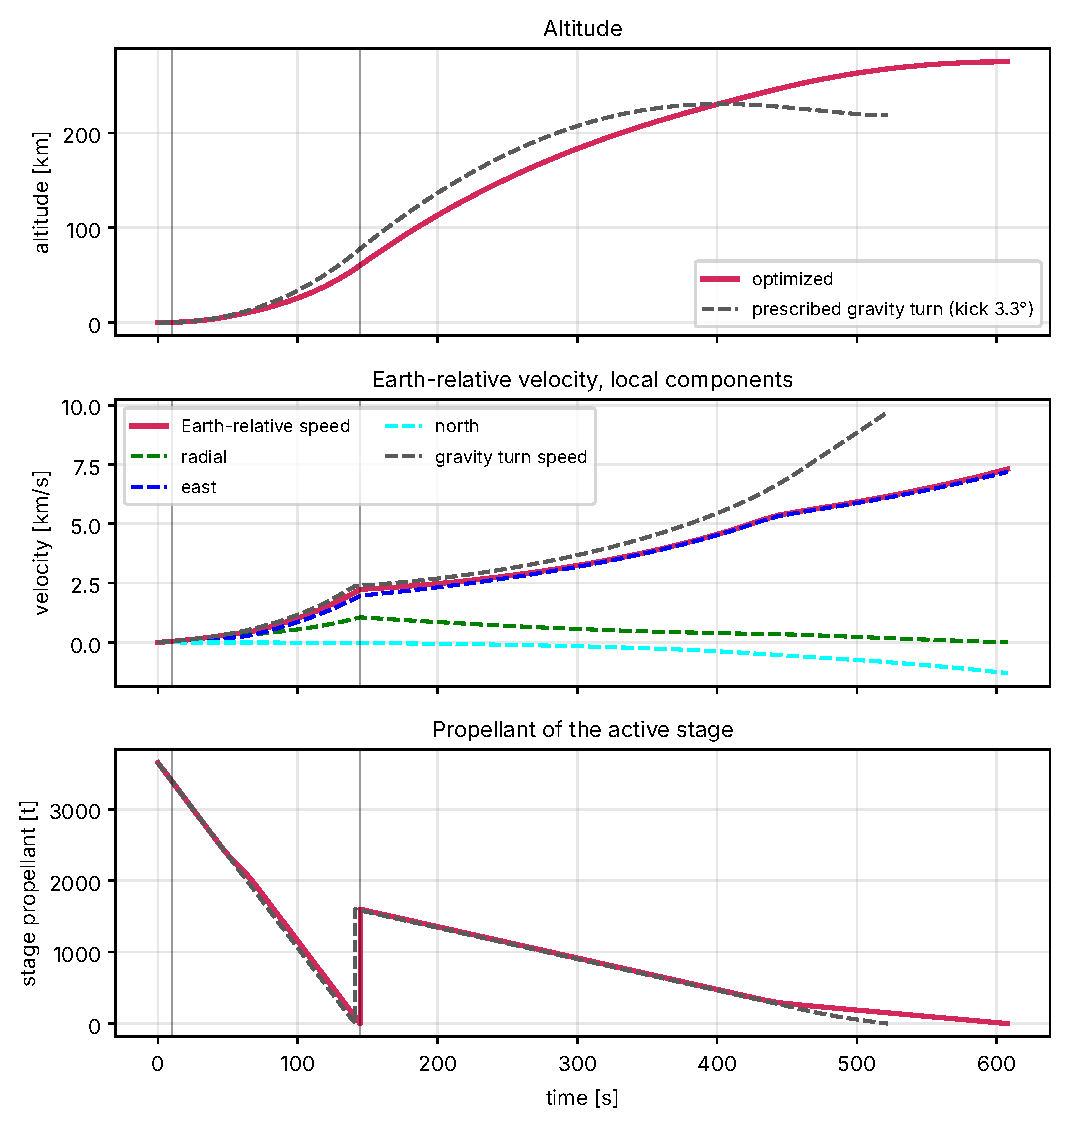
\includegraphics[height=0.8\textheight]{fig_hist_left}
    \end{column}
    \begin{column}{0.36\textwidth}
      \vspace{6pt}\small
      \begin{itemize}\setlength{\itemsep}{4pt}
        \item the gravity turn (kick \ang{3.3}) lofts to \SI{218}{km} with \SI{10.1}{km/s} -- \SI{2.4}{km/s} more than circular;
        \item the optimizer flies lower and flatter, inserts at exactly \SI{275}{km} / \SI{7740}{m/s}, and carries the difference as payload;
        \item both stages burn to zero reserve; staging at \SI{145}{s}.
      \end{itemize}
      \vspace{4pt}
      \stat{\SI{293.3}{\tonne}}{payload to \SI{275}{km} $\times$ \ang{26.0}, expendable trajectory, dry 200/100 t}
    \end{column}
  \end{columns}
\end{frame}

\begin{frame}{Baseline Solution -- Controls and Active Constraints}
  \framesubtitle{Both path constraints are active: max-$q$ in the booster burn, 4 $\gz$ at MECO}
  \begin{columns}[T]
    \begin{column}{0.62\textwidth}
      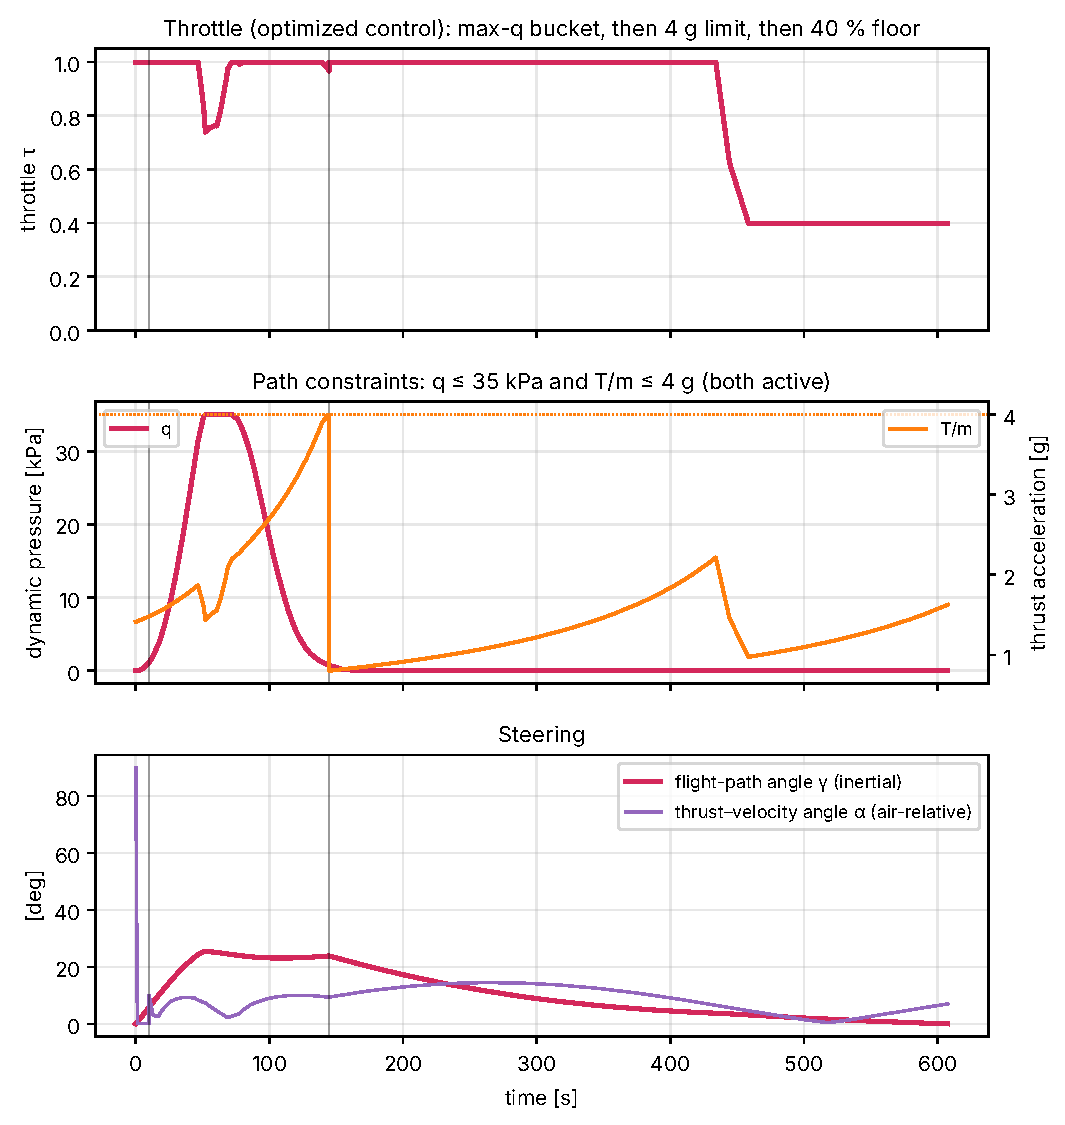
\includegraphics[height=0.8\textheight]{fig_hist_right}
    \end{column}
    \begin{column}{0.36\textwidth}
      \vspace{6pt}\small
      \begin{itemize}\setlength{\itemsep}{4pt}
        \item \textbf{max-$q$ bucket}: throttle to 0.74 between 50 and \SI{75}{s} holds $q=\SI{35}{kPa}$ exactly;
        \item \textbf{acceleration limit}: the booster reaches 4\,$\gz$ at MECO; the ship throttles to its 40\,\% floor for the last \SI{170}{s};
        \item \textbf{steering}: thrust pulls 10--\ang{15} off the air-relative velocity during the ship burn (the \SI{690}{m/s} steering loss) while $\gamma$ decays smoothly to zero.
      \end{itemize}
    \end{column}
  \end{columns}
\end{frame}

\begin{frame}{Baseline Solution -- the Numbers}
  \framesubtitle{Losses total \SI{1833}{m/s}: inside the textbook 1.5--2.0 km/s band, now decomposed}
  \begin{columns}[T]
    \begin{column}{0.3\textwidth}
      \stat{\SI{293.3}{\tonne}}{payload to \SI{275}{km} $\times$ \ang{26.0} (expendable trajectory, dry 200/100 t)}\\[8pt]
      {\color{PMS7635C}\textbf{\SI{145}{s} $\cdot$ \SI{60}{km} $\cdot$ \SI{2.61}{km/s}}}\\[-1pt]{\scriptsize\color{gray}staging (MECO), at the 4\,$\gz$ limit}\\[8pt]
      \stat{\SI{608}{s}}{insertion: $h$ \SI{275.000}{km}, $\gamma$ $5\!\times\!10^{-10}$ deg, \SI{7740.26}{m/s}}
    \end{column}
    \begin{column}{0.68\textwidth}
      \scriptsize
      \begin{tabular}{lr@{\quad}lr}
        \toprule
        \multicolumn{2}{l}{\textit{Trajectory}} & \multicolumn{2}{l}{\textit{$\dv$ budget (m/s)}} \\
        \midrule
        GLOW & \SI{5843}{\tonne} & $\dv_{vac}$ (both stages) & 9,155 \\
        max-$q$ (active) & \SI{35.0}{kPa}, 50--\SI{75}{s} & speed gained $|\bm v_f|-|\bm v_0|$ & 7,322 \\
        booster min throttle & 0.74 & gravity loss & 1,049 \\
        max $T/m$ (active) & 4.00\,$\gz$ at MECO & steering loss & 690 \\
        ship burn & \SI{463}{s}; $\tau=0.40$ last \SI{170}{s} & back-pressure loss & 76 \\
        inclination & \ang{25.997} (= latitude) & drag loss & 18 \\
        both stages & burn to zero reserve & $|\bm v_0|$ (rotation) & 418 \\
         & & identity residual & $-0.001$ \\
        \bottomrule
      \end{tabular}
      \vspace{6pt}

      \stepbox{3}{the losses are now computed for this vehicle and this orbit rather than taken from a band; the identity $\dv_{ideal}=v_{orbit}+\sum\text{losses}-v_{rot}$ closes to \SI{1}{mm/s}.}
    \end{column}
  \end{columns}
\end{frame}

\begin{frame}{The Same Vehicle Under a Prescribed Gravity Turn}
  \framesubtitle{Simulation vs.\ optimization: globe view and ascent profile}
  \centering
  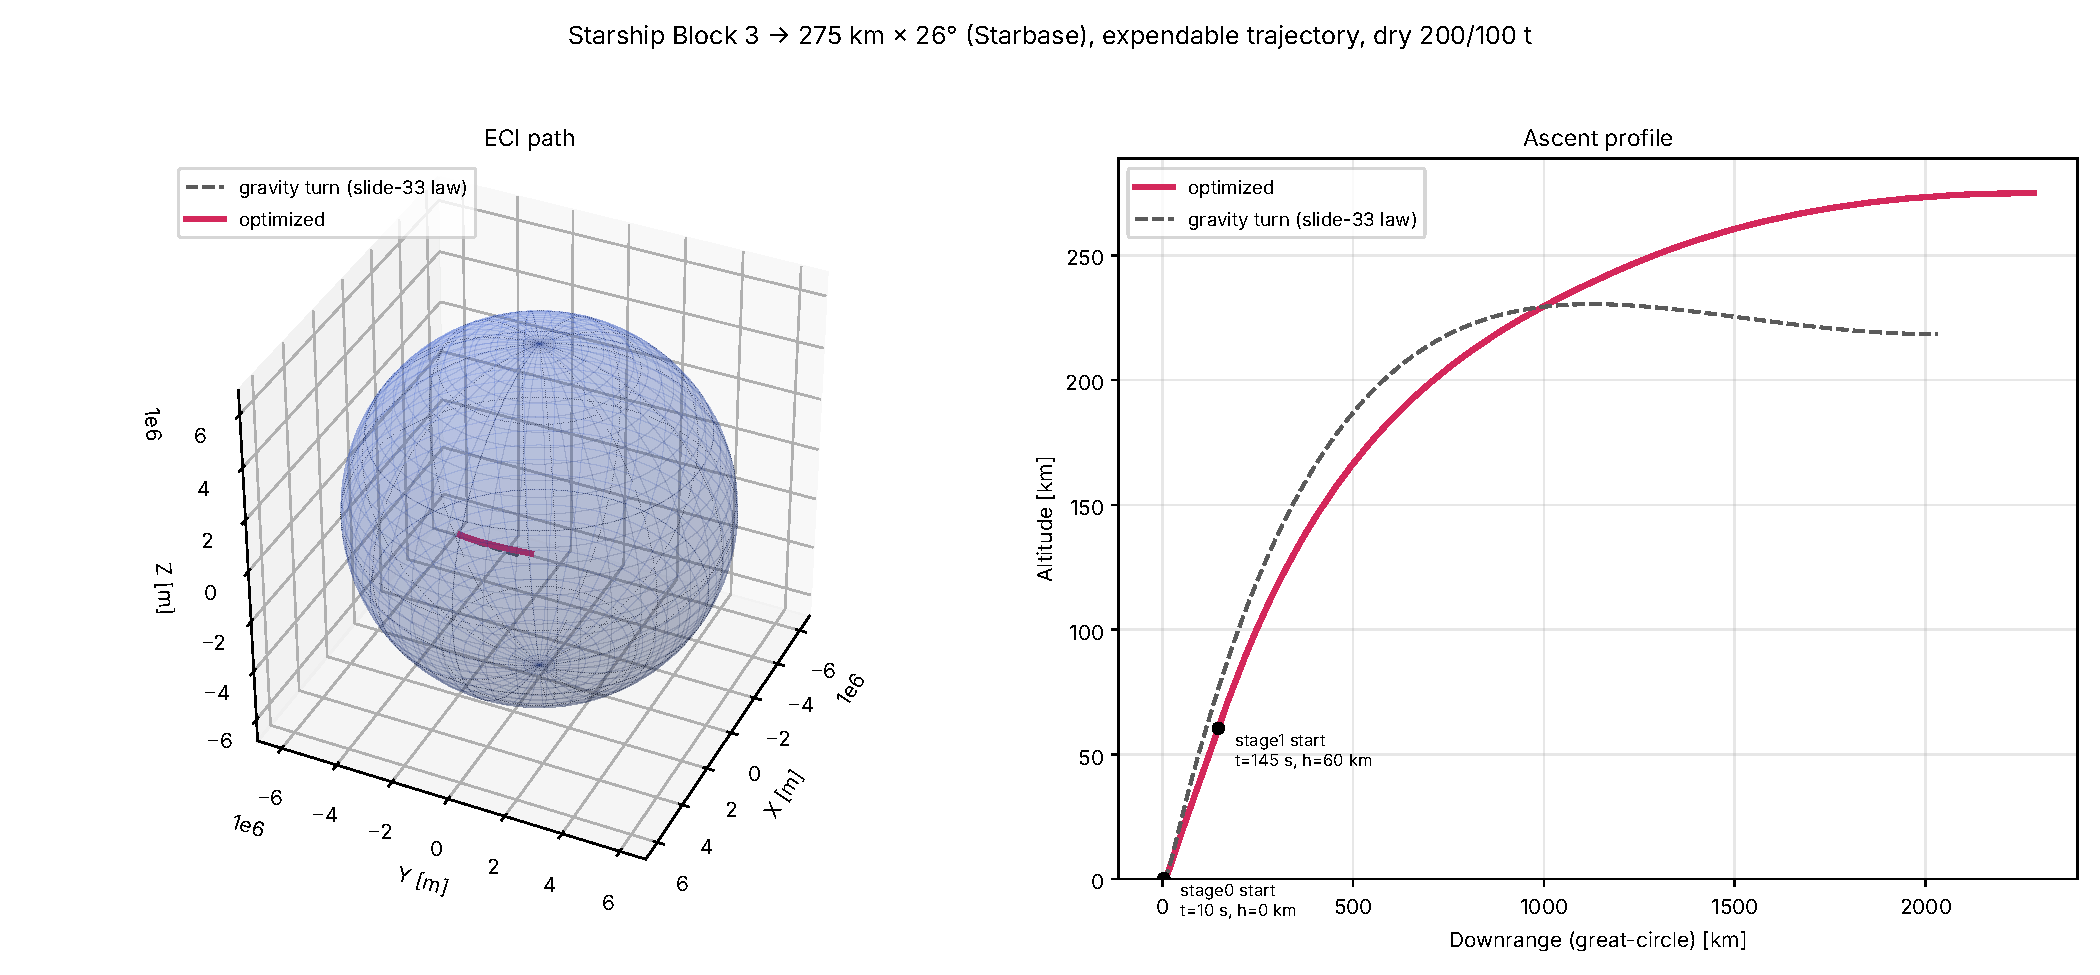
\includegraphics[width=0.88\textwidth]{fig_path3d}\\
  {\footnotesize The prescribed law reaches $\gamma=0$ at \SI{218}{km} with \SI{10.1}{km/s}: an eccentric orbit with \SI{2.4}{km/s} to spare. The optimizer inserts into the \SI{275}{km} circle and carries the difference as \SI{293}{\tonne} of payload.}
\end{frame}

\begin{frame}{The $\dv$ Budget, Closed Numerically}
  \framesubtitle{$\dv_{ideal}=v_{orbit}+\sum\text{losses}-v_{rot}$ -- computed instead of assumed}
  \centering
  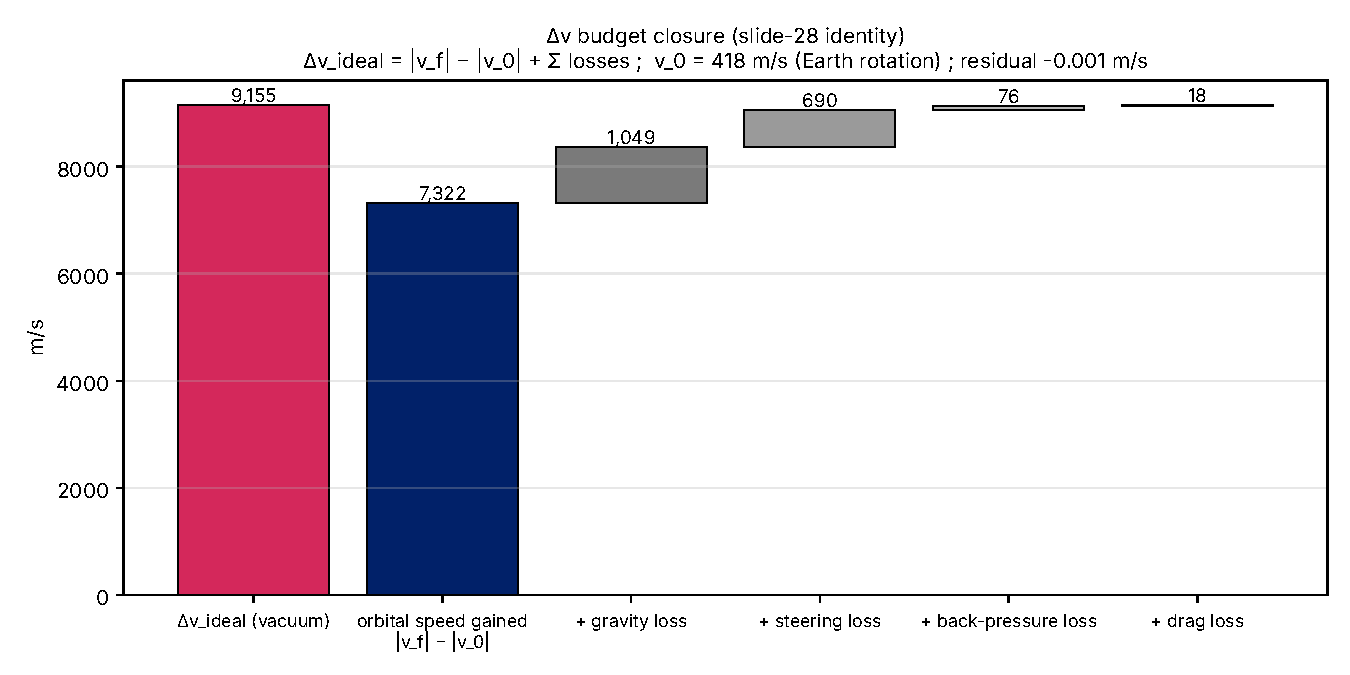
\includegraphics[width=0.84\textwidth]{fig_losses}\\
  {\footnotesize $\dv_{vac} = (|\bm v_f|-|\bm v_0|) + L_g + L_s + L_{bp} + L_D$ holds to \SI{-0.001}{m/s} because the five terms are integrated as states alongside the dynamics.}
\end{frame}

\begin{frame}{Propulsion Requirements Handed to the Thrust-Chamber and Cycle Steps}
  \framesubtitle{Per stage: $T_{vac}$, throttle profile, $\Isp(h)$, $\mdot$, burn time, propellant}
  \centering
  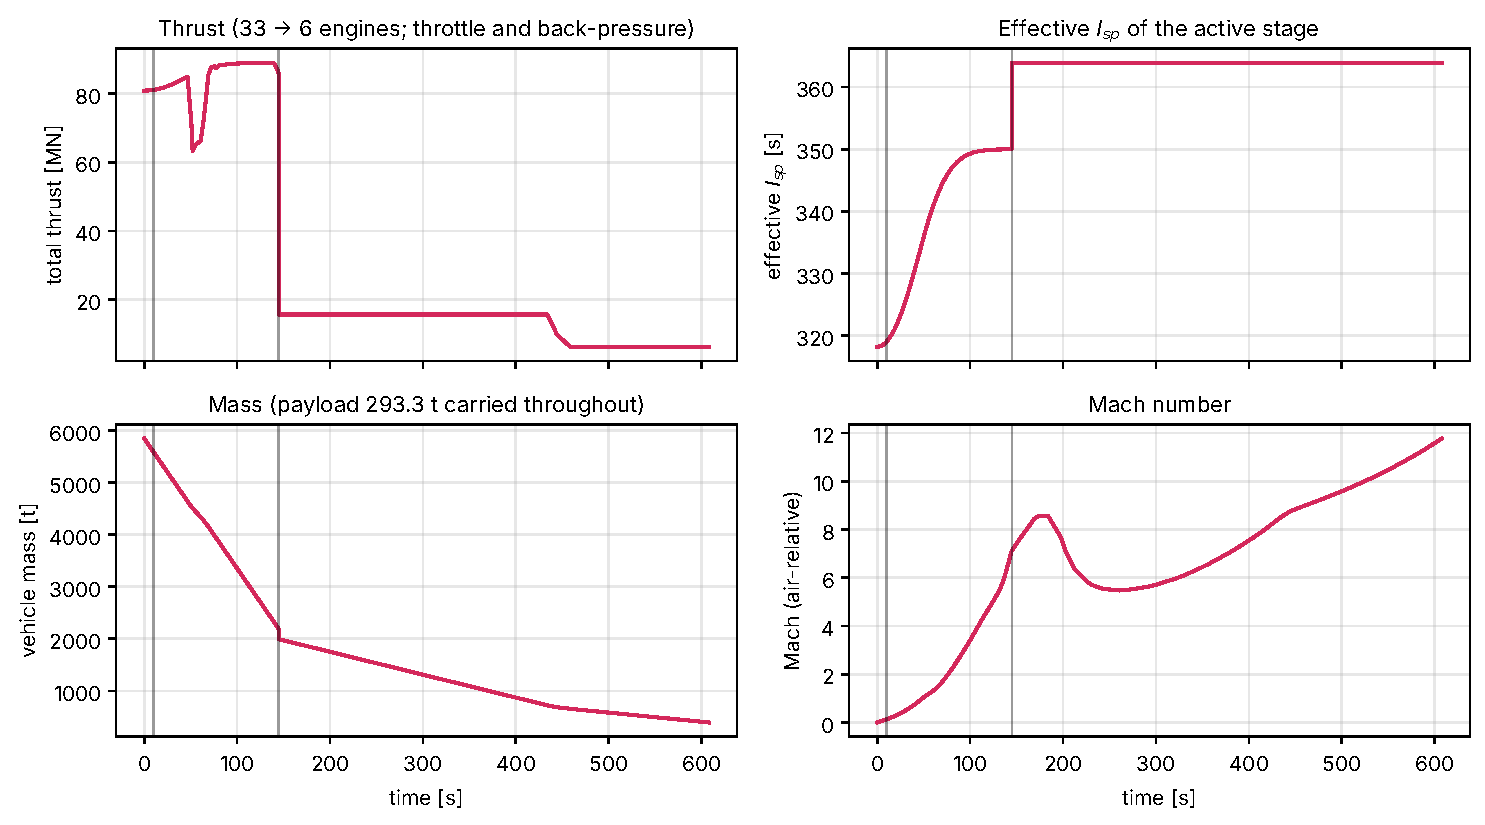
\includegraphics[height=0.58\textheight]{fig_thrust_isp_mass}
  \stepbox{5--8}{these are the inputs to thrust-chamber design and to cycle / turbopump design; the $\Isp$ rise in the first \SI{60}{s} is the back-pressure term, the step at \SI{145}{s} is staging onto the Raptor~3 / RVac set (thrust-weighted \SI{363.9}{s}).}
\end{frame}

\begin{frame}{What the Optimizer Chose: Steering}
  \framesubtitle{Pitch-over through the max-$q$ bucket, then a near-linear pitch program; no out-of-plane steering}
  \centering
  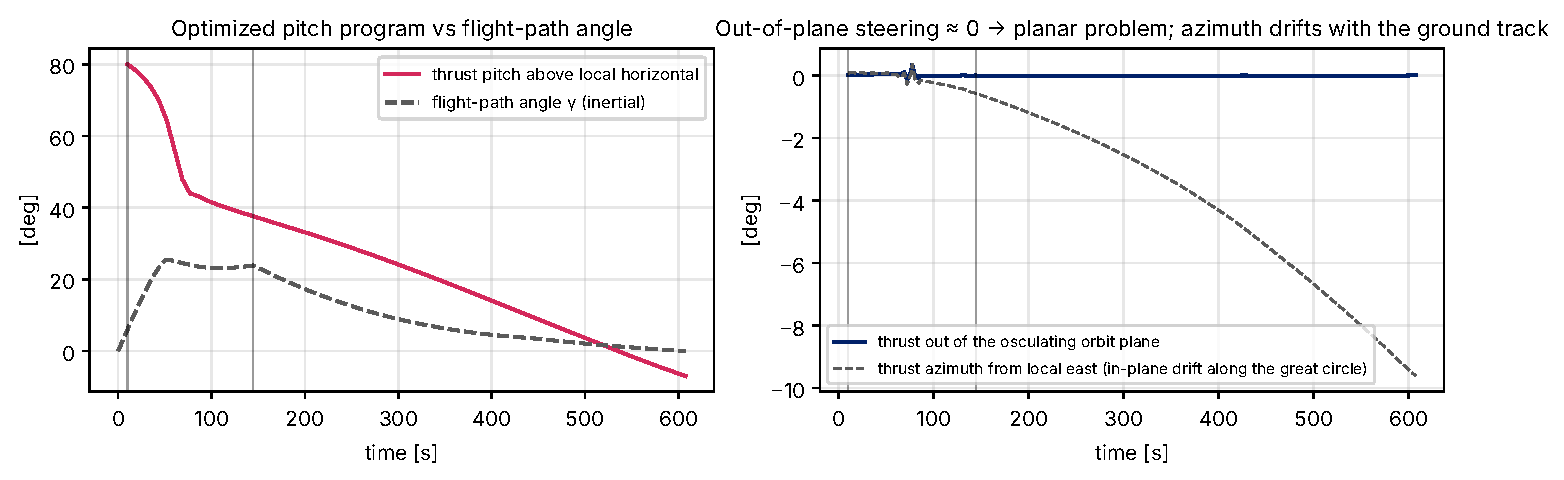
\includegraphics[width=\textwidth]{fig_steering}\\
  {\footnotesize Pitch to $\sim$\ang{45} by the end of the max-$q$ bucket, then down to slightly negative at insertion. The thrust component out of the osculating orbit plane is zero: the optimizer discovers that an eastward launch is a planar problem; the azimuth drifts only because the ground track leaves the \ang{26}N apex of the orbit.}
\end{frame}

% =====================================================================
\section{Sensitivities}
\begin{frame}{What the Published 100 t Depends On}
  \framesubtitle{Seven cases from the baseline by command-line deck overrides, each warm-started from the previous solution}
  \centering
  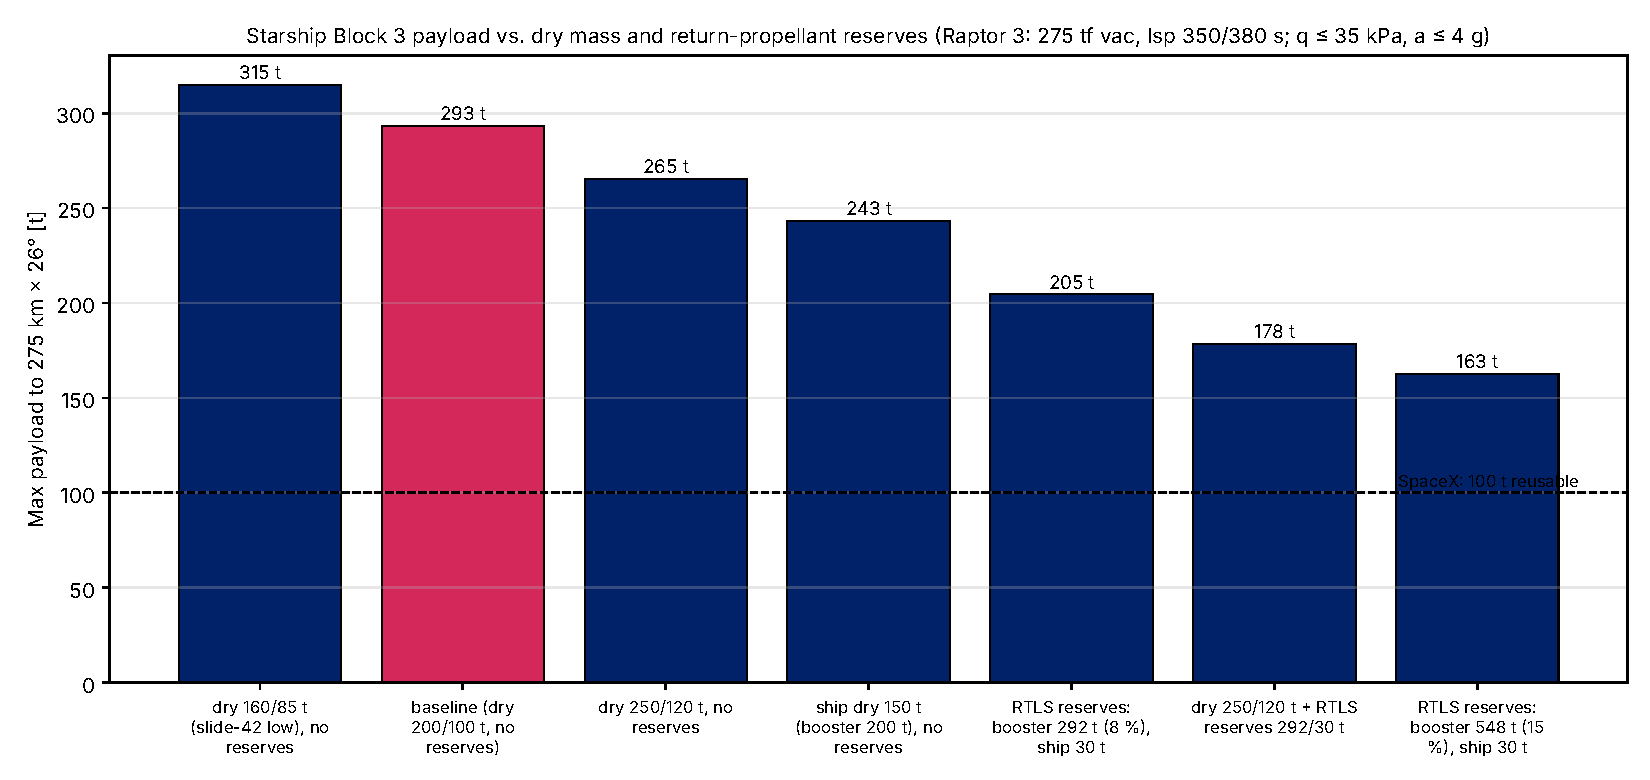
\includegraphics[width=0.9\textwidth]{fig_sweep}
\end{frame}

\begin{frame}{Sensitivities}
  \framesubtitle{Ship dry mass 1:1, booster dry mass 0.16:1, reserves the largest lever}
  \centering
  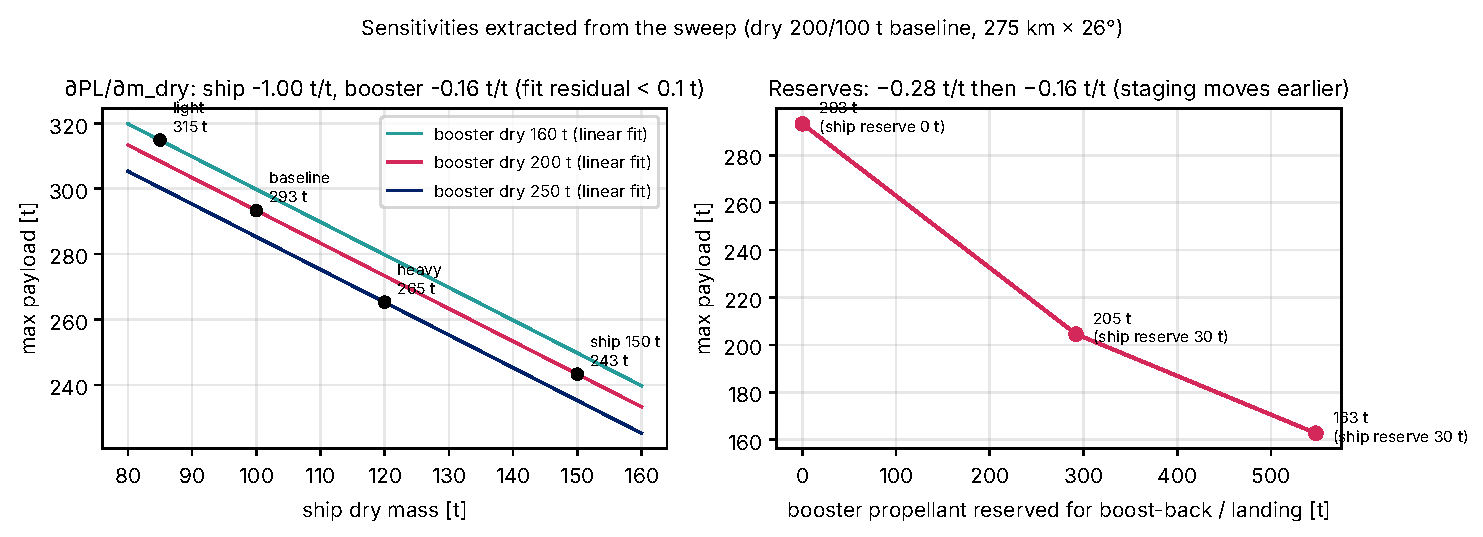
\includegraphics[width=\textwidth]{fig_sensitivity}
  \begin{columns}[T]
    \begin{column}{0.5\textwidth}
      \footnotesize $m_{pay} = 425.8 - 0.161\,m_{dry,booster} - 1.001\,m_{dry,ship}$ [t] reproduces the four no-reserve cases to \SI{0.07}{\tonne}: a kilogram on the ship is a kilogram of payload; on the booster, \SI{160}{g}.
    \end{column}
    \begin{column}{0.5\textwidth}
      \footnotesize 8\,\% of booster propellant held back + \SI{30}{\tonne} in the ship costs \SI{89}{\tonne}; 15\,\% costs \SI{131}{\tonne}. The optimizer re-stages earlier on its own -- the mechanism behind ``stage low for reusability''.
    \end{column}
  \end{columns}
\end{frame}

\begin{frame}{Reserves Move the Staging Point}
  \framesubtitle{Same max-$q$ bucket; MECO moves earlier and lower and the ship carries more of the $\dv$}
  \centering
  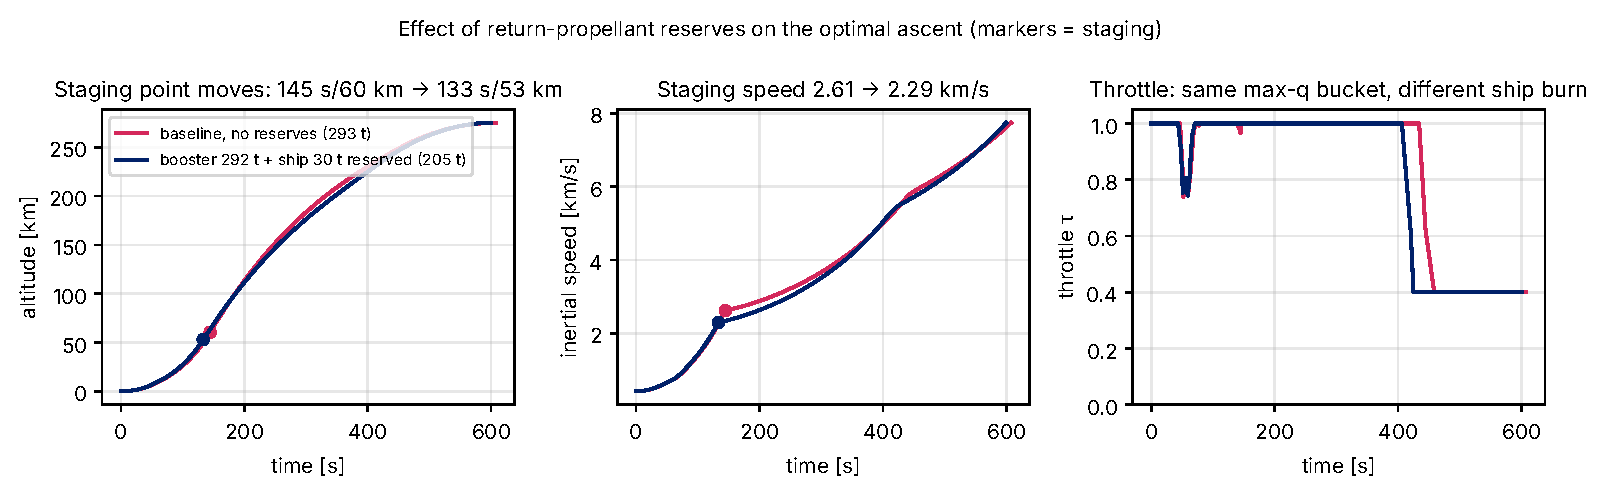
\includegraphics[width=\textwidth]{fig_reserve_compare}\\
  {\footnotesize MECO: \SI{145}{s} / \SI{60}{km} / \SI{2.61}{km/s} (no reserves) $\to$ \SI{133}{s} / \SI{53}{km} / \SI{2.29}{km/s} (8\,\%) $\to$ \SI{123}{s} / \SI{47}{km} / \SI{2.00}{km/s} (15\,\%).}
  \src{IFT-3 public timeline: hot staging at T+2:50, \SI{72}{km}, on a flown return-to-site profile (Cit\'e de l'espace)}
\end{frame}

\begin{frame}{Where the Remaining Gap to 100 t Lives}
  \framesubtitle{The pessimistic corner (dry 250/120 t + 8\,\% reserve) still gives \SI{178}{\tonne}}
  \begin{columns}[T]
    \begin{column}{0.5\textwidth}
      \begin{block}{What the model carries}
        \begin{itemize}
          \item published propellant loads and Raptor 3 performance
          \item dry masses (swept 160--250 / 85--150 t)
          \item return-propellant allowances (0--15\,\% booster, \SI{30}{\tonne} ship)
          \item max-$q$ and acceleration limits, throttle floor
          \item gravity, drag, steering and back-pressure losses -- computed, not assumed
        \end{itemize}
      \end{block}
    \end{column}
    \begin{column}{0.5\textwidth}
      \begin{block}{What it does not carry (yet)}
        \begin{itemize}
          \item actual ship dry mass with heat shield and flaps (likely $>\SI{120}{\tonne}$) -- 1:1 on payload
          \item boost-back propellant that grows with staging speed and must fly a \emph{specific} return trajectory
          \item engine margins, $C_D(M)$, $J_2$, winds, 6-DOF
          \item operational and performance margins
        \end{itemize}
      \end{block}
    \end{column}
  \end{columns}
  \vspace{6pt}
  \centering
  The tool's contribution is not the number -- it is that the gap is now a list of named quantities with known sensitivities.
\end{frame}

% =====================================================================
\section{Verification}
\begin{frame}{Verification}
  \framesubtitle{What was actually checked (9 Nov 2026)}
  \begin{columns}[T]
    \begin{column}{0.58\textwidth}
      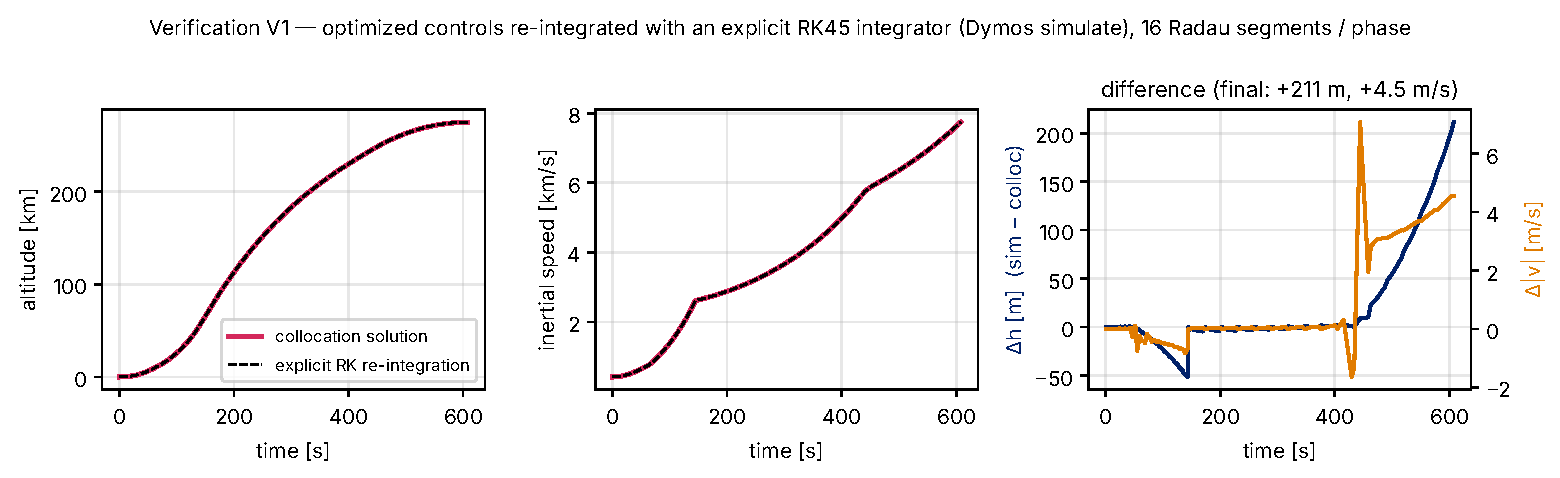
\includegraphics[width=\textwidth]{fig_verification}
    \end{column}
    \begin{column}{0.42\textwidth}
      \footnotesize
      \begin{tabular}{p{2.3cm}p{3.3cm}}
        \toprule
        check & result \\
        \midrule
        Dymos SSTO benchmark & $t_f$ \SI{143.77}{s}, 27 iter.\ (doc $\approx$\SI{143}{s}) \\
        explicit re-integration & $+\SI{211}{m}$, $+\SI{4.5}{m/s}$ (16 seg.); $+\SI{322}{m}$, $+\SI{8.8}{m/s}$ (12 seg.) \\
        grid independence & \SI{293.20}{\tonne} vs \SI{293.31}{\tonne} \\
        loss identity & $\le\SI{0.004}{m/s}$, all 7 cases \\
        jax partials vs FD & $\sim10^{-10}$ \\
        US76 vs \texttt{ambiance} & $<0.1\,\%$ to \SI{81}{km} \\
        rocket-equation consistency & optimizer's $\dv_{vac}$ in the hand method returns \SI{293.3}{\tonne} \\
        \bottomrule
      \end{tabular}
    \end{column}
  \end{columns}
  \vspace{3pt}
  {\footnotesize The re-integration drift starts at the \SI{440}{s} throttle transition, where the piecewise control is least accurate; it halves from 12 to 16 segments.}
  \src{Dymos documentation: SSTO Earth-launch example (Longuski Titan II)}
\end{frame}

\begin{frame}{Limitations and What Comes Next}
  \framesubtitle{Known limits of v0.1 and the two remaining milestones}
  \begin{columns}[T]
    \begin{column}{0.5\textwidth}
      \begin{block}{Known limits of v0.1}
        \begin{itemize}
          \item constant $C_D$; no $J_2$, winds, 6-DOF
          \item reserves are inputs; the return flight is not simulated
          \item the ship's final 40\,\%-throttle arc should be re-checked with grid refinement and another initial guess
          \item a ``Falcon-9-like'' single-stage test vehicle ($T/W$ 3.75, 95\,\% propellant fraction) does not converge as a max-payload problem -- $\approx\SI{0}{\tonne}$ at 79\,$\gz$; not a useful test case
        \end{itemize}
      \end{block}
    \end{column}
    \begin{column}{0.5\textwidth}
      \begin{block}{Milestones}
        \begin{itemize}
          \item \textbf{by 11/19} -- $C_D(M)$, $J_2$, grid refinement; in-space $\dv$ module (Hohmann / Lambert, $C_3$, aerocapture) feeding the terminal set for the Mars, Moon and Titan missions
          \item \textbf{by 12/3} -- co-design: engine group from $(\pc,\eps,O/F)$ via $\cstar$, $\CF$; stage mass model; dry masses and loads as design variables
          \item then -- FFSC-cycle / turbopump models as OpenMDAO components in the same problem (why Dymos)
        \end{itemize}
      \end{block}
    \end{column}
  \end{columns}
\end{frame}

\begin{frame}[fragile]{Running It}
  \framesubtitle{conda environment, one command per case, warm starts and deck overrides for sweeps}
\begin{lstlisting}
conda env create -f environment.yml && conda activate ascentopt     # cyipopt must be present
python scripts/run_case.py --vehicle vehicles/starship_v3_baseline.yaml --out runs/starship \
    --h-target 275e3 --lat 25.997 --q-max 35e3 --a-max 39.2266 --segments 16 --max-iter 400 --simulate
python scripts/run_case.py ... --out runs/heavy --warm-from runs/starship/*_out/dymos_solution.db \
    --set stage0.dry_mass=250e3 --set stage1.dry_mass=120e3
python scripts/make_figures.py runs/starship --out results/figs
bash reproduce_demo.sh           # baseline + six-case sweep + figures, 15-25 min
\end{lstlisting}
  \begin{columns}[T]
    \begin{column}{0.5\textwidth}
      \footnotesize
      \textbf{Stack:} OpenMDAO 3.41, Dymos 1.16, pyoptsparse 2.17 + cyipopt 1.7 / Ipopt 3.14, jax 0.7 -- conda-forge + PyPI.\\
      \textbf{Deck:} YAML -- engines (anchor pair + exit area), stages (dry, propellant, reserve, engine sets), diameter, $C_D$.
    \end{column}
    \begin{column}{0.5\textwidth}
      \footnotesize
      \textbf{Outputs:} \texttt{result.json} (payload, staging, losses, constraint activity, simulate check), Dymos record for warm starts and plots, time-history / path / loss / steering figures.\\
      \textbf{Repository:} \texttt{Modern-Aerospace-Propulsion/Week 10 - Mission Analysis/ascentopt/} -- fixed-vehicle mode now; co-design mode to follow.
    \end{column}
  \end{columns}
\end{frame}

\begin{frame}{Summary}
  \framesubtitle{From a forward simulation to a design tool}
  \begin{itemize}\setlength{\itemsep}{5pt}
    \item \tool\ turns the ascent simulation into an optimizer: same physics, steering and throttle solved for, stages as linked phases, orbit as a constraint, payload as the objective.
    \item Starship Block 3 to \SI{275}{km} $\times$ \ang{26}: \textbf{\SI{293}{\tonne}} on an expendable trajectory with 200/100 t dry masses; losses \textbf{\SI{1833}{m/s}}, decomposed; max-$q$ and 4\,$\gz$ limits both active; staging at \SI{145}{s} / \SI{60}{km} / \SI{2.61}{km/s}.
    \item Sensitivities from a seven-case sweep: ship dry mass \textbf{1:1}, booster dry mass 0.16:1, 8\,\% booster reserve $-\SI{89}{\tonne}$ with the staging point moving on its own.
    \item Verified: benchmark reproduced, explicit re-integration within \SI{211}{m} / \SI{4.5}{m/s}, grid-independent to 0.04\,\%, $\dv$ identity closed to \SI{1}{mm/s}.
    \item Next: $C_D(M)$ and the in-space module for the project missions; then propulsion co-design in the same NLP.
  \end{itemize}
\end{frame}

\end{document}
